\chapter{Discussion ESB in Openshift}
\label{cha:esbd}
This chapter will evaluate the implemented prototype of Chapter \vref{cha:esbi}, and will show that challenges such as
\begin{itemize}
	\item managing multiple environments,
	\item managing service security,
	\item managing multiple service versions,
	\item managing public API migration,
	\item and managing adapters and transformers as services
\end{itemize}
are manageable tasks when hosting an ESB in Openshift. Whenever possible, Openshift will be compared to JBoss EAP, which is used as the platform for ESB middleware as discussed in Section \vref{fig:esb-software-architecture}.

\section{Managing Multiple Environments}
\label{sec:esbd-multiple-env}
An ESB is commonly hosted on multiple environments, whereby at least one productive and one testing environment should be present. These environments where commonly a VM, which provides the runtime environment for the ESB. As the prototype shows, the environment is now represented by an Openshift Project, which can be reproduced easily via scripts as discussed in Section \vref{sec:esbi-openshift}. \\

The services hosted on the ESB are using Fuse integration Service 2.0 and its provided tooling, which ensure that the services are properly encapsulated in a container and properly managed in Openshift. Therefore, the service developers provide the necessary Openshift Templates, which has the effect, that the operators have no interaction with the service artifacts and runtime environments anymore. Operator have only to manage
\begin{itemize}
	\item the Openshift Project, which hosts the services,
	\item the Openshift ConfigMaps, which hold the service non-sensitive configuration,
	\item the Openshift Secrets, which hold the sensitive service configuration,
	\item and scripts for utility such as backup/restore of service data or instance scaling.
\end{itemize} 
\ \\
Listing \vref{ls:esboi-config-project-stages-prod} shows how developers reference Openshift Objects such as Openshift ConfigMaps and Openshift Secrets, which are managed by operators. 

Figure \vref{fig:esbd-multi-stage-env} illustrates the management and provisioning of multiple environments for an ESB, whereby the hosting environment is represented by an Openshift Project. The \mentionedtext{Management Server} pulls the scripts and Openshift Templates from a \mentionedtext{VCS Server} and the configurations from a \mentionedtext{Configuration Server}, and uses them to provision new Openshift Projects or manage existing ones. \\

The scripts and Openshift Templates are separated from the configurations, which are actually providing the data for the scripts and Openshift Template-Parameters. With such an approach, the infrastructure becomes reproducible, versioned, and therefore consistent, and disposable. These characteristics are also principles of IaC, which have been discussed in Chapter \vref{cha:iac}. 

\begin{figure}[htbp]
	\centering
	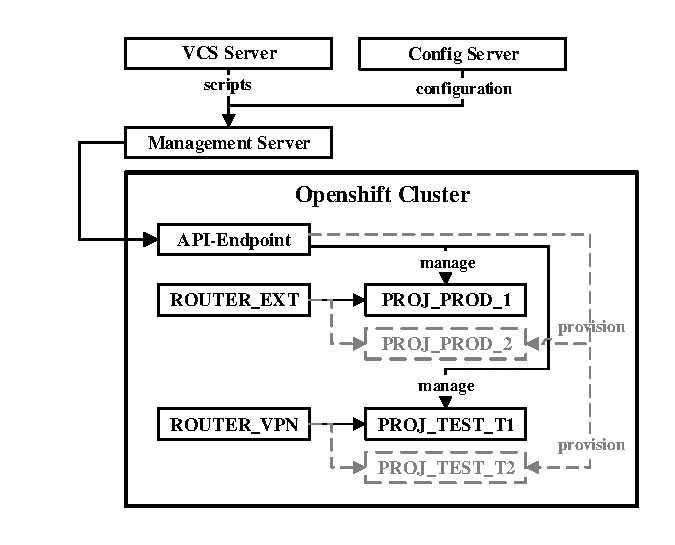
\includegraphics[scale=1]{images/esbd-multi-stage-env.pdf}
	\caption{Management and provisioning of multiple environments}
	\label{fig:esbd-multi-stage-env}
\end{figure}

The interaction of the \mentionedtext{Management Server, VCS Server} and \mentionedtext{Configuration Server} as illustrated in Figure \vref{fig:esbd-multi-stage-env}, is similar to the Figure \vref{fig:reproduce-infrastructure}, which illustrated how a system can be reproduced with parametrized templates and an IaC tool. The Openshift CLI provides functionality to manage Openshift Objects, which is what needs to be done when providing an environment in form of an Openshift Project, therefore the Openshift CLI acts as an IaC tool.  \\

Table \vref{tab:esbd-multi-stage-env} illustrates what mechanisms Openshift and JBoss EAP contain to provide the listed infrastructure features. As illustrated in Table \vref{tab:esbd-multi-stage-env}, Openshift provides \mentionedtext{Networking} and \mentionedtext{Isolation} features, which are provided to JBoss EAP by its hosting environment, such as a VM. Except of the \mentionedtext{Networking} and \mentionedtext{Isolation} feature, JBoss EAP supports all other features either natively or by supporting a third party framework. Nevertheless, Openshift combines all features in one platform, and makes them easy manageable via Openshift Templates and the Openshift CLI.

{\renewcommand{\arraystretch}{1.2}%
\begin{table}[h]
	\begin{tabularx}{\textwidth}{ X|X|X }	
	  \textbf{Feature}              & \textbf{Openshift}      & \textbf{JBoss EAP} \\  \hline
	  \textit{Staging}                  & Openshift Project       & Server Instance \\  \hline
	  \textit{Management}               & Openshift CLI           & JBoss CLI \\
	                                    & Openshift Web-Console   & JBoss Web-Console \\
	                                    & Openshift REST-API      & \\  \hline
	  \textit{Networking}               & Openshift Project       & None (external) \\
	                                    & Openshift Service       & \\  
	                                    & Openshift Route         & \\  \hline
	                                    & Openshift Router        & \\  \hline
	  \textit{Isolation}                & Openshift Project       & None (external) \\  \hline
	  \textit{Configuration/Secrets}    & Openshift ConfigMaps    & Java System Properties  \\
	                                    & Openshift Secrets       & Environment variables \\
	                                                             && Password Vault \\  \hline
	  \textit{Service Distribution}     & Openshift Worker-Node   & Single JVM \\ 
			                                                     && Karaf \\  
			                                                     && OSGI \\  \hline
	  \textit{Service Roll-out}         & Recreate                & Framework dependent, \\ 
			                            & Rolling                 & normally recreate \\
	\end{tabularx}
	\caption{Infrastructure feature comparison}
	\label{tab:esbd-multi-stage-env}
\end{table}}

Openshift runs Docker Containers, and therefore the programming language, the service was implemented with, does not matter, because the Docker Container provides the runtime environment for the application. Also services hosted on PaaS platforms communicate via standard Protocols such as Http, which are commonly supported by almost any programming language. JBoss EAP on the contrary, runs only Java applications. \\ 

The next section will discuss the service security within an Openshift Project, which can be managed as discussed in this section. Additionally to the by the Openshift design provided security, the \mentionedtext{Management Server} of Figure \vref{fig:esbd-multi-stage-env} could also manage custom security configurations, which can be managed via the Openshift CLI as well. 

\section{Managing Service Security}
\label{sec:esbd-service-security}
With a common ESB middleware, the services are protected by running within a single runtime environment or by security features provided by an supported third party framework like Karaf. In an Openshift Project, the services are implicitly protected by being isolated in a Kubernetes Namespace as discussed in Section \vref{sec:paas-openshift-project}, which can not be accessed by other Openshift Projects without additional configuration.

\begin{figure}[htbp]
	\centering
	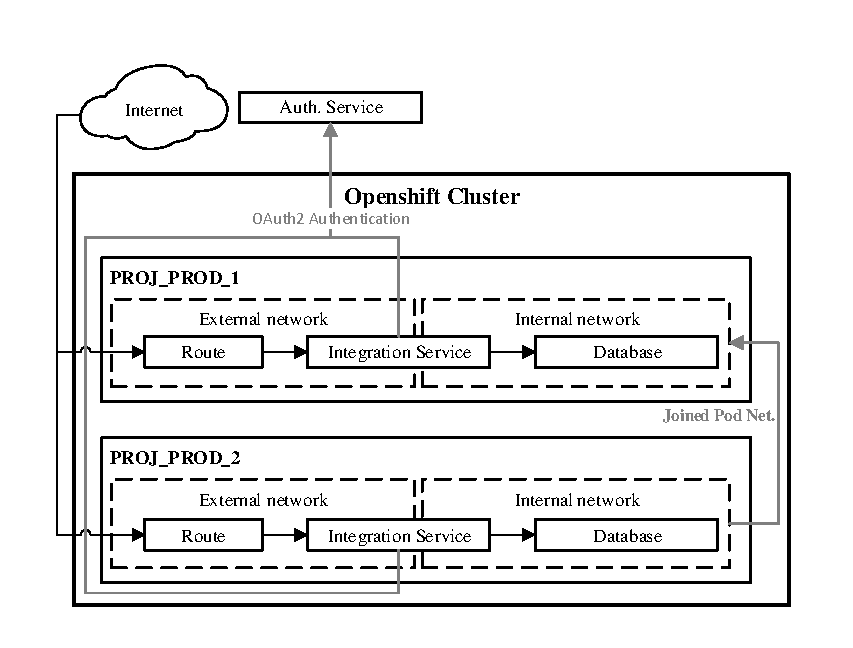
\includegraphics[scale=1]{images/esbd-service-security.pdf}
	\caption{Service security in an Openshift Project}
	\label{fig:esbd-service-security}
\end{figure}
\ \\
Figure \vref{fig:esbd-service-security} illustrates an example, similar to the implemented prototype, where two Openshift Projects host the same services and where the Pod Networks of the two Openshift Projects are joined. The illlustrated configured joined Pod Networks allow services hosted in project \mentionedtext{PROJ\_PROD\_2} to access services hosted in project \mentionedtext{PROJ\_PROD\_1}. The default is, that all Openshift Projects are isolated. This kind of configuration is performed by Openshift Cluster-Administrators, and cannot be performed by developers. \\

Additionally to the isolation of the services within the Openshift Project, the \mentionedtext{Integration Services} are secured via OAuth2, whereby the resource access is controlled by a central \mentionedtext{Single-Sign-On Server (SSO Server)}. On the one hand the services are isolated within a Kubernetes Namespace, and on the other hand, additional security such as resource access control can provided by the service itself as discussed in Section \vref{sec:esbi-security}. It is not meant to isolate services from each other within an Openshift Project, because an Openshift Project or a Kubernetes Namespace should contain a set of service, which do not have to be isolated from each other. \\

Table \vref{tab:esbd-service-security} illustrates what mechanism Openshift and JBoss EAP contain to provide the listed security features. As illustrated in Table \vref{tab:esbd-service-security}, Openshift does not provide any support for access control on the service level, which is normal for an PaaS platform such as Openshift. The services running in Docker Containers on an Openshift Cluster have to implement access control or have to use third party frameworks such as Wildfly Swarm, which provide access control features as discussed in Section \vref{sec:esbi-security}. JBoss EAP on the other hand is a Java Application-Server, which provides support for resource access or user control for several common providers. 

{\renewcommand{\arraystretch}{1.2}%
	\begin{table}[h]
		\begin{tabularx}{\textwidth}{ X|X|X }	
			\textbf{Feature}                 & \textbf{Openshift}      & \textbf{JBoss EAP} \\  \hline
			\textit{Network Isolation}       & Openshift Project       & None (VM) \\  \hline
			\textit{HTTPS}                   & Openshift Router        & Reverse Proxy \\
			                                 & Openshift Route         & Endpoint Configuration \\  \hline
            \textit{Access Control}          & None (external)         & Endpoint Configuration \\
                                                                      && Internal User-Database \\ 
                                                                      && External User-Database \\  \hline
            \textit{Single-Sign-On}          & None (external)         & Endpoint Configuration \\
                                                                      && Several SSO providers \\  \hline
		\end{tabularx}
		\caption{Security feature comparison}
		\label{tab:esbd-service-security}
\end{table}}

Openshift does not provide access control features to secure service resources, but provides security features such as user/group/role management, project permission management, Pod Network management, or quota management for Openshift Objects such as Replication Controllers. The security is applied to the services in an ambient way, whereby the services for instance don't have to support HTTPS anymore, because within an Pod Network there is no need for additional security and exposed services have an Openshift Route, which acts as the reverse proxy for the service, which handles security. All Openshift security configurations outside the scope of an Openshift Project can only be performed by Openshift Cluster-Administrators. 
\newpage

\section{Managing Multiple Service Versions}
\label{sec:esbd-multi-version-service}
Sometimes it is necessary to run multiple versions of a service, for instance if a new version is released or if a consumer is not capable of migrating to the new version but provides a significant business value for the enterprise. The Openshift Platform provides mechanisms to run multiple versions of a service in several ways. Figure \vref{fig:esbd-service-multiple-versions} illustrates some scenarios for running multiple service versions on Openshift, whereby the illustrated scenarios of \mentionedtext{PROJ\_1} and \mentionedtext{PROJ\_2} are possible, because the old service version is N-1 compatible. N-1 compatibility means, that the service in the old version is capable of reading data written by the service in the new version. \\

\begin{figure}[htbp]
	\centering
	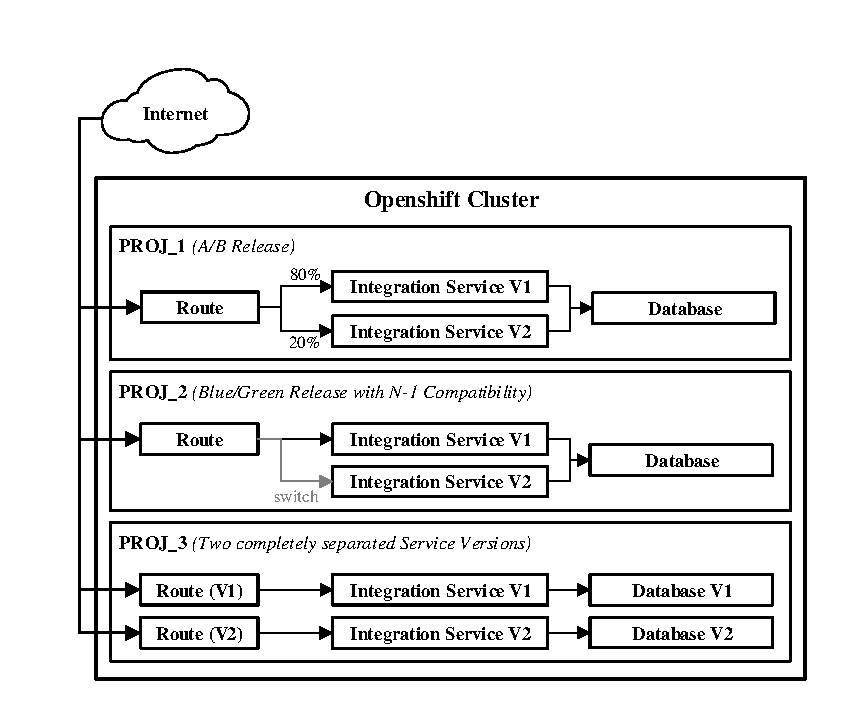
\includegraphics[scale=1]{images/esbd-service-multiple-versions.pdf}
	\caption{Running multiple service versions on Openshift}
	\label{fig:esbd-service-multiple-versions}
\end{figure}
\ \\
\emph{PROJ\_1} of Figure \vref{fig:esbd-service-multiple-versions} illustrates an A/B Release, which is used to run the old and new version of a service in parallel, whereby a portion of the service consumers get access to the new version, while the rest of the service consumers are still using the old version. A/B Releases are used to validate the new version in the productive environment, before fully releasing it to all consumers. In this scenario, the requests are load balanced with the defined weightings, to either the new or old service version. \\ 

\emph{PROJ\_2} of Figure \vref{fig:esbd-service-multiple-versions} illustrates a Blue/Green Release, which is used to run the old and the new version of a service in parallel, whereby the Openshift Route switches between the old and new service version. In this scenario, all service consumer access the same service version, which is currently accessible by the Openshift Route. \\

\emph{PROJ\_3} of Figure \vref{fig:esbd-service-multiple-versions} illustrates two service versions running completely separated in parallel, whereby both versions are accessible via their own Openshift Route. This scenario is not a release scenario, and should be used if multiple service versions have to be provided outside of the scope of a release. \\

Table \vref{tab:esbd-service-multiple-versions} illustrates what mechanism Openshift and JBoss EAP contain to provide the listed release features. Multiple service versions on Openshift are represented by separate Openshift Service objects, whereby with JBoss EAP, multiple service versions are either represented by separate JBoss EAP instances or deployment contexts on a single JBoss EAP instance.

{\renewcommand{\arraystretch}{1.2}%
 \newcolumntype{m}{>{\hsize=.32\hsize}X}%
	\begin{table}[h]
		\begin{tabularx}{\textwidth}{ X|X|X }	
			\textbf{Feature}                  & \textbf{Openshift}      & \textbf{JBoss EAP} \\  \hline
			\textit{Multiple Service Versions}& Openshift Service       & Multiple EAP instances \\
																	   && Multiple deployment contexts \\ \hline
			\textit{Weighted Routing}         & Openshift Route         & None (external) \\  \hline
			\textit{Version Switch}           & Openshift Route         & None (external) \\  \hline
		\end{tabularx}
		\caption{Release feature comparison}
		\label{tab:esbd-service-multiple-versions}
\end{table}}

JBoss EAP is an application platform for Java applications, which provides an runtime environment for applications but no networking features as shown in Table \vref{tab:esbd-multi-stage-env}, and therefore no routing feature. JBoss EAP can be configured to act as a reverse proxy, but cannot act as the reverse proxy for applications hosted on the same JBoss EAP instance. \\

As Figure \vref{fig:esbd-service-multiple-versions} illustrates, the implemented prototype can run multiple versions of the hosted services, and supports the implementation of release models such as A/B or Blue/Green Releases. nt release models.
\newpage

\section{Managing Migration of Public API}
\label{sec:esbd-multi-stage-env}
This section will discuss the management of services public API, which is crucial when it comes to distributed services. Changes made on the public API of a service can break the functionality of an application the service is part of, or break the functionality of an external application, which depends on this service. The public API is the API the service exposes, which could only be consumed by internal consumers, but has to be managed the same way as the API would be exposed to external consumers. There are several ways to migrate a public API, whereby some of them will be discussed in this section. \\  

Services running on Openshift are completely separated from each and have their own life-cycle, therefore they have to provide a public API, which can be consumed by other services. The public API has to be designed properly in the first place, as well as the management of its migrations. At least, the last both versions will have to be supported, to give the developers of the consuming services enough time to apply to the migrations of the public API. Commonly a service has two versions, on the one hand the service release version and on the other hand the service API version, which is allowed to remain the same over multiple service releases. \\

The following sections will discuss the different ways to version the public API of a service.

\mysubsubsection{Query Parameter-Versioning}
Multiple versions of a public API can be managed via a Query-Parameter, whereby the Query-Parameter defines the version to use of a single API Operation. The URL \inlineBash{http://localhost/api/users?version=2} illustrates how to access a specific version of an API Operation via a HTTP Query-Parameter. The following Table \vref{tab:esbd-service-api-query-param} shows the Pros and Cons of API Versioning with HTTP Query-Parameters.

{\renewcommand{\arraystretch}{1.2}%
	\begin{table}[h]
		\begin{tabularx}{\textwidth}{ X|X }	
			\textbf{Pros}                 & \textbf{Cons}    \\  \hline
			Single resource address       & Data and control parameters are mixed     \\  
			Supported by all browsers     & Version as data parameter not possible     \\
			Easy to understand            & No declarative mapping with JAX-RS     \\
			Easy to implement             & \\ \hline
		\end{tabularx}
		\caption{Pros and Cons of HTTP Query-Parameter Versioning}
		\label{tab:esbd-service-api-query-param}
\end{table}}

\mysubsubsection{HTTP Header Versioning}
Multiple version of a public API can be managed via HTTP Headers in the following listed ways:
\begin{itemize}
	\item New HTTP Header \\
	e.g. \inlineBash{Version: 2}
	\item Additional field in the Accept-Header \\
	e.g. \inlineBash{Accept: application/json; version=2}
	\item Enhanced Media-Type \\
	e.g. \inlineBash{Accept: application/vnd.app.model.v1+json;qs=0.9}
\end{itemize}
\ \\
The approach of HTTP Header Versioning brings in more flexibility, but also makes the API Versioning more complex for developers to implement and harder to understand for consumers. The following Table \vref{tab:esbd-service-api-http-header} shows the Pros and Cons of API Versioning with HTTP Headers.

{\renewcommand{\arraystretch}{1.2}%
	\begin{table}[h]
		\begin{tabularx}{\textwidth}{ X|X }	
			\textbf{Pros}                         & \textbf{Cons}    \\  \hline
			Single resource address               & Header handling needed     \\  
			No mix of data and control parameters & Harder to implement/understand     \\
			Declarative mapping with JAX-RS       & No enhanced Media-Type in HTML     \\
			Easy to implement                     & More difficult to test \\ \hline
		\end{tabularx}
		\caption{Pros and Cons of HTTP Header Versioning}
		\label{tab:esbd-service-api-http-header}
\end{table}}

\mysubsubsection{Path Versioning}
The easiest way to manage multiple versions of a public API is Path Versioning, whereby the whole API is versioned, instead of single API Operations. The URL \inlineBash{http://localhost/api/v2/users} illustrates how to access a specific version of an API Operation via a Path version. The Path Versioning is the most used approach to version a public API, because of its simplicity to realize.  The following Table \vref{tab:esbd-service-api-path} shows the Pros and Cons of API Versioning with Path versions.

{\renewcommand{\arraystretch}{1.2}%
	\begin{table}[h]
		\begin{tabularx}{\textwidth}{ X|X }	
			\textbf{Pros}                         & \textbf{Cons}    \\  \hline
			Easy to implement                     & Multiple resource addresses      \\
			Easy to understand                    & Version actually not part of resource     \\  
			No mix of data and control parameters & Latest version unknown \\ \hline
		\end{tabularx}
		\caption{Pros and Cons of Path Versioning}
		\label{tab:esbd-service-api-path}
\end{table}}

\section{Managing Adapters and Transformers as Services}
\label{sec:esbd-adap-trans-service}


\section{Further Work}
\label{sec:esbd-furhter-work}